\documentclass[times, utf8, zavrsni]{fer}
\usepackage[titletoc]{appendix}
\usepackage{booktabs}
\usepackage{graphicx}
\usepackage[]{algorithm2e}
\usepackage{caption}
\usepackage{multirow}
\usepackage{listings}
\usepackage{xcolor}
\usepackage{textcomp}
\definecolor{listinggray}{gray}{0.9}
\definecolor{lbcolor}{rgb}{0.9,0.9,0.9}
\lstset{
	backgroundcolor=\color{lbcolor},
	tabsize=4,    
	%   rulecolor=,
	language=[GNU]C++,
	basicstyle=\scriptsize,
	upquote=true,
	aboveskip={1.5\baselineskip},
	columns=fixed,
	showstringspaces=false,
	extendedchars=false,
	breaklines=true,
	prebreak = \raisebox{0ex}[0ex][0ex]{\ensuremath{\hookleftarrow}},
	frame=single,
	numbers=left,
	showtabs=false,
	showspaces=false,
	showstringspaces=false,
	identifierstyle=\ttfamily,
	keywordstyle=\color[rgb]{0,0,1},
	commentstyle=\color[rgb]{0.026,0.112,0.095},
	stringstyle=\color[rgb]{0.627,0.126,0.941},
	numberstyle=\color[rgb]{0.205, 0.142, 0.73},
	%        \lstdefinestyle{C++}{language=C++,style=numbers}’.
}
\lstset{
	backgroundcolor=\color{lbcolor},
	tabsize=4,
	language=C++,
	captionpos=b,
	tabsize=3,
	frame=lines,
	numbers=left,
	numberstyle=\tiny,
	numbersep=5pt,
	breaklines=true,
	showstringspaces=false,
	basicstyle=\footnotesize,
	%  identifierstyle=\color{magenta},
	keywordstyle=\color[rgb]{0,0,1},
	commentstyle=\color{Darkgreen},
	stringstyle=\color{red}
}
\graphicspath{{/home/mateo/Git/Kraken_memory_improvement/Pictures/}}
\begin{document}

% TODO: Navedite broj rada.
\thesisnumber{5133}

% TODO: Navedite naslov rada.
\title{Algoritam staničenja velike baze podataka genoma}

% TODO: Navedite vaše ime i prezime.
\author{Mateo Stjepanović}

\maketitle

% Ispis stranice s napomenom o umetanju izvornika rada. Uklonite naredbu \izvornik ako želite izbaciti tu stranicu.
\izvornik

% Dodavanje zahvale ili prazne stranice. Ako ne želite dodati zahvalu, naredbu ostavite radi prazne stranice.
\zahvala{Zahvaljujem mentorici doc.\ dr.\ sc.\ Mirjana Domazet-Lošo na podršci.}

\tableofcontents

\chapter{Uvod}
Bioinformatika je interdisciplinarna znanost koja se bavi razvojem programa i metoda za interpretiranje bioloških podataka. Spaja matematiku, statistiku, računalnu znanost te druge prirodno matematičke znanosti. U posljednjem desetljeću bioinformatika kao znanost doživaljava veliki porast, te kao takva uspjeva mapirati genome mnogih živih bića.\\
U navedenom porastu najviše se ističu metode analiziranja genoma, te, spajanjem statističkih analiza i algoritama iz područja računalne znanosti, metode određivanja položaja istih u taksonomskom stablu. Upravo u tom području postoje mnogi alati koji su razvijeni upravo s ciljem poboljšanja točnosti određivanja taksonomskog stabla novoj, nepoznatoj, jedinki.\\ Za većinu jedinki u uzorku su vrsta, rod i više razine stabla nepoznati. Ako je jedinka potpuno nepoznata tada će se klasificirati kao nova nepoznata vrsta te se neće dalje klasificirati. U velikom broju slučajeva će postojati neke sličnosti sa nekim već određenim vrstama, te je potrebno pronaći te sličnosti kako bi se sjedinka uspješno klasificirala. Za to služe razni algoritmi poravnanja. Jedan od tih je BLAST. Postoje druge metode i programi koji pospješuju učinkovitost BLAST-a uvođenjem metoda strojnog učenja. Iako bolje preciznosti ti programi imaju jednu veliku manu. Vrijeme potrebno za klasificiranje podatka je jako veliko, stoga su više manje neiskoristivi. \\Tu na scenu nastupa alat za klasifikaciju metagenoma nazvan Kraken(Derrick E. Wood i Steven L.).
\\{\textit{Kraken is ultrafast and high accurate program for assigning taxonomic labels to metagenomic DNA sequences.}\footnote[1]{Wood and Salzberg: \textbf{Kraken: ultrafast metagenomic sequence classification using exact alignments.} \textit{Genome Biology} 2914 15:R46}
\\Za razliku od alata koji su pokušali poboljšati preciznost BLAST algoritma, te time izgubili na brzini, Kraken je jedan od rijetkih alata koji postiže točnost koja premašuje onu u BLAST algoritmu, s time da ne gubi na brzini izvođenja. Rad Krakena se sastoji od toga da se ulazni podatak "razbija" na k-mere, te se minimizer algoritmom traže oni k-meri koji imaju istu vrijednost minimzer-a. Tada se taj podatak uspoređuje s podacima u Kraken-ovoj bazi podataka, s tim da je baza sortirana na način da su podaci sa istim minimizerom smješteni jedan pored drugog, tako da se pretraživanje jako pospješuje i ubrzava. Autori alata su shvatili da Kraken može naići an problem prilikom izvođenja na računalu s ograničenim resursima, točnije na računalu s RAM-om ispod 70GB. Iz tog razloga je razvijena MiniKraken baza podataka koja je sa prvotnih 70GB podataka smanjena na 4GB.
\begin{table}[htb]
	\centering
	\resizebox{\textwidth}{!}{%
		\begin{tabular}{|llcccccc|}
			\hline
			\multicolumn{1}{|c}{} & \multicolumn{1}{c}{}  & \multicolumn{2}{c}{HiSeq}                                       & \multicolumn{2}{c}{MiSeq}                                       & \multicolumn{2}{c|}{simBA-5}                                     \\
			\multicolumn{2}{|l}{Classifier}              & \multicolumn{1}{l}{Precision} & \multicolumn{1}{l}{Sensitivity} & \multicolumn{1}{l}{Precision} & \multicolumn{1}{l}{Sensitivity} & \multicolumn{1}{l}{Precision} & \multicolumn{1}{l|}{Sensitivity} \\ \hline
			Megablast             & \multicolumn{1}{l|}{} & \multicolumn{1}{c|}{99.03}    & \multicolumn{1}{c|}{79.00}      & \multicolumn{1}{c|}{92.44}    & \multicolumn{1}{c|}{75.76}      & \multicolumn{1}{c|}{96.93}    & 93.67                            \\ \hline
			NBC                   & \multicolumn{1}{l|}{} & \multicolumn{1}{c|}{82.33}    & \multicolumn{1}{c|}{82.33}      & \multicolumn{1}{c|}{77.78}    & \multicolumn{1}{c|}{77.78}      & \multicolumn{1}{c|}{97.64}    & 97.64                            \\ \hline
			PhymmBL               & \multicolumn{1}{l|}{} & \multicolumn{1}{c|}{79.14}    & \multicolumn{1}{c|}{79.14}      & \multicolumn{1}{c|}{76.21}    & \multicolumn{1}{c|}{76.21}      & \multicolumn{1}{c|}{96.11}    & 96.11                            \\ \hline
			PhymmBL65             & \multicolumn{1}{l|}{} & \multicolumn{1}{c|}{99.13}    & \multicolumn{1}{c|}{73.95}      & \multicolumn{1}{c|}{92.47}    & \multicolumn{1}{c|}{73.03}      & \multicolumn{1}{c|}{99.08}    & 95.45                            \\ \hline
			Kraken                & \multicolumn{1}{l|}{} & \multicolumn{1}{c|}{99.20}    & \multicolumn{1}{c|}{77.15}      & \multicolumn{1}{c|}{94.71}    & \multicolumn{1}{c|}{73.46}      & \multicolumn{1}{c|}{99.90}    & 91.25                            \\ \hline
			Kraken-Q              & \multicolumn{1}{l|}{} & \multicolumn{1}{c|}{99.12}    & \multicolumn{1}{c|}{76.31}      & \multicolumn{1}{c|}{94.69}    & \multicolumn{1}{c|}{70.41}      & \multicolumn{1}{c|}{99.92}    & 89.54                            \\ \hline
			MiniKraken            & \multicolumn{1}{l|}{} & \multicolumn{1}{c|}{99.44}    & \multicolumn{1}{c|}{66.12}      & \multicolumn{1}{c|}{97.41}    & \multicolumn{1}{c|}{67.95}      & \multicolumn{1}{c|}{99.95}    & 65.87                            \\ \hline
			MiniKraken-Q          & \multicolumn{1}{l|}{} & \multicolumn{1}{c|}{99.36}    & \multicolumn{1}{c|}{65.67}      & \multicolumn{1}{c|}{97.32}    & \multicolumn{1}{c|}{65.84}      & \multicolumn{1}{c|}{99.98}    & 65.31                            \\ \hline
			Kraken-GB             & \multicolumn{1}{l|}{} & \multicolumn{1}{c|}{99.51}    & \multicolumn{1}{c|}{93.75}      & \multicolumn{1}{c|}{98.48}    & \multicolumn{1}{c|}{86.23}      & \multicolumn{1}{c|}{99.48}    & 91.13                            \\ \hline
		\end{tabular}%
	}
	\caption{Klasifikacija roda za tri metagenoma}
	\label{StatRez}
\end{table}

Iz tablice 1.1 ,koja predstavlja rezultate izvođenja na 3 seta metagenoma, se može vidjeti kako Kraken prednjači u preciznosti svoje klasifikacije. Iako je osjetljivost nešto manja nego u Megablast-a, program koji radi na implementaciji BLAST algoritma za poravnanje, ta razlike je nezamjetna. Tablica prikazuje i neke druge alate, te Kraken alat sa raznim opcijama i na raznim bazama podataka. Kraken-Q predstavlja izvedbu Krakena sa uključenom opcijom \textit{quick}, koja doprinosi brzini izvođenja. MiniKraken je Kraken program koji se izvodi na MiniKraken bazi podataka. Ona je stvorena iz originalne baze podataka tako da se uklanja svaki k-ti element iz nje.

\chapter{Definiranje problema}
Uz već spomenutost rješenja problema korištenja velike količine resursa, nailazi se na problem koji će se pokušati riješiti tijekom ovog rada.
% Please add the following required packages to your document preamble:
% \usepackage{graphicx}
\begin{table}[hbp]
	\centering
	\resizebox{\textwidth}{!}{%
		\begin{tabular}{|llcccccc|}
			\hline
			\multicolumn{1}{|c}{} & \multicolumn{1}{c}{} & \multicolumn{2}{c}{HiSeq} & \multicolumn{2}{c}{MiSeq} & \multicolumn{2}{c|}{simBA-5} \\
			\multicolumn{2}{|l}{Classifier} & \multicolumn{1}{l}{Precision} & \multicolumn{1}{l}{Sensitivity} & \multicolumn{1}{l}{Precision} & \multicolumn{1}{l}{Sensitivity} & \multicolumn{1}{l}{Precision} & \multicolumn{1}{l|}{Sensitivity} \\ \hline
			Kraken & \multicolumn{1}{l|}{} & \multicolumn{1}{c|}{99.20} & \multicolumn{1}{c|}{77.15} & \multicolumn{1}{c|}{94.71} & \multicolumn{1}{c|}{73.46} & \multicolumn{1}{c|}{99.90} & 91.25 \\ \hline
			MiniKraken & \multicolumn{1}{l|}{} & \multicolumn{1}{c|}{99.44} & \multicolumn{1}{c|}{66.12} & \multicolumn{1}{c|}{97.41} & \multicolumn{1}{c|}{67.95} & \multicolumn{1}{c|}{99.95} & 65.87 \\ \hline
		\end{tabular}%
	}
	\caption{Isječak iz Tablice 1.1}
	\label{IsjecakTablice}
\end{table}

Iako se iz dane tablice vidi da se preciznost korištenjem MiniKraken baze podataka neznatno povećala u odnosu na Kraken bazu podataka. S druge strane osjetljivost jako opada. \\Osjetljivost predstavlja mjeru koja određuje postotak uočenih lažno negativnig podataka, tj. predstavlja postotak točno kvalificiranih podataka koji su uistinu tako i predstavljeni. S druge strane precizonst predstavlja izbjegavanje lažno pozitivnih podataka, tj. koliko podataka je uočeno da ne pripadaju nekoj skupini, s tim da oni uistinu ne pripadaju toj skupini.\\Ideja ovog rada je da se algoritmima sličnim algoritmima straničenja osposobi računalo s ograničenim resursima za rad s bazom podataka čija veličina uvelike nadilazi količinu RAM-a raspoloživog na računalu. Prvotno je potrebno podjeliti bazu podataka na više manjih cjelina koje će se moći uspješno učitati u memoriju te pretražiti. Ideja je iskoristiti "kontejnere" k-mera koji su određeni svaki jedinstvenom minimizer vrijednosti, te pomoću binarnog pretraživanja indeksa učitavati samo onu bazu podataka pomoću koje je moguće klasificirati podatak u taksonomsko stablo. Želeći se približit straničenju, predstavit će se samo iteriranje po indeksima, te će se učitavanje i pretraživanje svake od baze podataka vršiti slijedno.
\chapter{Strukture podataka i algoritmi u Kraken-u}
\subsection{Baza podataka}
\subsubsection{Kreiranje baze podataka}

Nastanak baze podataka se odvija u nekoliko koraka. Za početak se sa NCBI-ove stranice preuzimaju biblioteke koje sadrže podatke i genome trenutno poznatih vrsta. Naravno nije potrebno sve podatke, nego se može preuzeti samo jedno carstvo ili samo jedan podskup podataka od kojih će se graditi baza podataka. Budući da pretraživanje baze podataka u Kraken-u osniva na k-merima potrebno je proizvesti k-mere za svaki podataka u bazi podataka. Za to služi alat naziva Jellyfish(Guillaume Marçais i Carl Kingsford) koji računa k-mere zadane duljine 31 ( korisnik također može zadati duljinu k-mera).\\Jellyfish je alat za brzo i memorijski povoljno prebrojavanje podnizova u danom nizu. Za potrebe prilagodbe svim resursima za Jellyfish postoje opcije za brzo izračunavanje koje je memorijski zahtjevnije, te ono sporije ali memorijski ne toliko zahtjevno. U kontekstu bioinformatike Jellyfish se koristi za prebrojavanje k-mera u zadanom metagenomu. Sam rad se bazira na hash tablici koja je osposobljena za paralelan rad preko više CPU-a. Hash tablica se sastoji od para (ključ,vrijednost), gdje je ključ zadani k-mer a vrijednost je broj njegovog ponavljanja u metagenomu.
	 	
\begin{table}[hbp]
	\centering
	\caption{Prikaz niza te njegovih k-mera (k = 4)}
	\label{Prikaz k-mera}
	\begin{tabular}{llllllllll}
		Ulaz:  &           & \multicolumn{8}{l}{AGATCGAGTG}                            \\
		4-mer: & \multicolumn{2}{l}{} & AGAT & GATC & ATCG & TCGA & CGAG & GAGT & AGTG
	\end{tabular}
\end{table}
Nakon rada Jellyfish-a u bazu se spremaju 4 bajtne vrijednosti k-mera te se kreira identifikacijska oznaka za svaki podataka. Tada program kreiranja baze podataka ponovno prolazi kroz istu, te za svaki identifikator podatka izračunava njegov LCA(\textit{Najmanji zajednički predal}), te ga sprema u bazu podataka zajedno s identifikatorom i njegovim k-merima.
\subsubsection{Strukture baze podataka}
Gore navedeni proces klasificiranja ulaznog genoma pomoću baze podataka se , već navedeno, bazira na pretraživanju k-mera. Baza podataka se sastaoji od identifikacijskih oznaka svakog podatka u njoj, njihovog izračunatog najmanjeg zajedničkog pretka, te k-mera koje on tvori.\\
\begin{figure}[hbp]
	\centering
	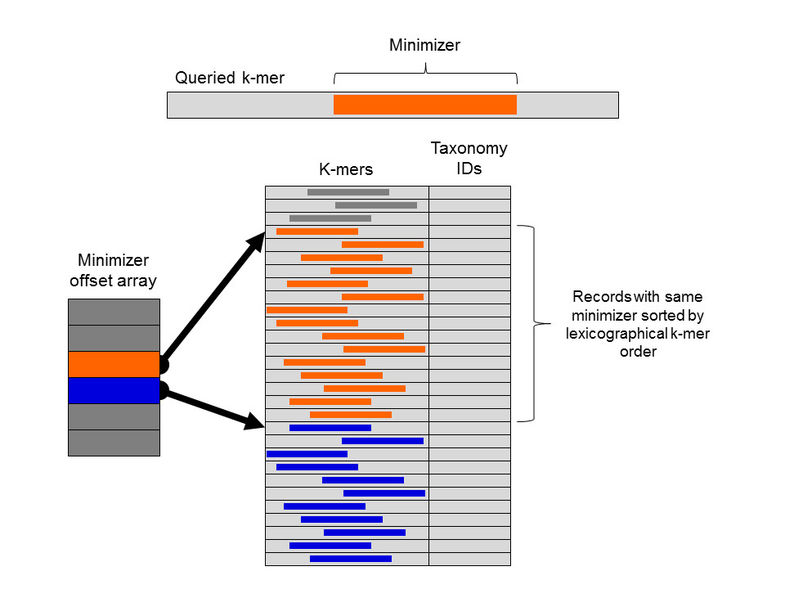
\includegraphics[width=\textwidth]{DbStructure.jpg}
	\caption{Prikaze strukture baze podataka}
	\label{BazaPodataka}
\end{figure}

S ciljem poboljšanja brzine pretraživanja, uvodi se algoritam indeksiranja i raspoređivanja poznat pod imenom Minimizer (Roberts M, Hayes W, Hunt B, Mount S, i Yorke J.). Računanje indeksa kontejnera je odvije kroz dvije petlje. U prvoj petlji se iterira po broju kontejnera te se za svaki od njih pohvaća njihov jedinstveni k-mer. Na osnovu njega se računa ključ te se popunjava niz brojem podataka koji ulaze u taj indeks. Nakon toga se računa ofset svih podataka te se zbrajaju s onim podacima koji se nalaze u nizu indeksa. Na kraju se iz varijable ofset kreira indeks vanjskom funkcijom.
 
\begin{figure}
	\begin{algorithm}[H]
		\SetAlgorithmName{Algoritam}{algoritam}{List of algoritam}
		ptr <- pokazivač\_na\_k-mer\;
		k\_ct <- brojač kontejnera\;
		vrijednosti <- 1ull << (nt * 2)\;
		\While{brojač je različit od broja kontejnera}{
			brojač++\;
			dohvati\_k-mer(ptr)\;
			ključ <- izračunaj\_ključ()\;
			b\_brojac[ključ]++\;		
		}
		b\_ofset[vrijednosti +1]\;
		\For{i < vrijednosti}{
			b\_ofset = b\_ofset[i-1]+b\_brojac[i-1]\;
		}
		indeks(b\_ofset)\;
		\caption{Računanje indeksa kontejnera}
		\label{Indeks}
	\end{algorithm}
\end{figure}


Prilikom sortiranja i indeksiranja se stvaraju svojevrsni kontejneri u bazu podataka slijedno sadržavaju one podatke čiji k-meri imaju iste minimizer vrijednosti. Podaci u svakom kontejneru su leksikografski poredani kako bi se isti osposobio za daljnje binarno pretraživanje. Stvaranjem zasebnih kontejnera se poboljšava pretraživanje na način da se za svaki ulazni podataka računaju njegovi k-meri te njegove minimizer vrijednosti, te se pretragom liste indeksa dohvaća samo onaj kontejner koji sadrži istu minimizer vrijednost. Prilikom dolaska novog podataka minimizer vrijednost se ne računa odmah, nego se prvo vrši pretraga na kontejneru na kojem smo već pozicionirani. Ako se podatak ne nalazi u zadanom kontejneru, tada se prelazi na računanje minimizer vrijednosti. Ako je minimizer vrijednost ista kao i kod kontejnera tada se podatak svrstava u neklasificirane te sa svaka daljnja klasifikacija zaustavlja, s druge strane pozicionira se na indeks izračunatog kontejnera te vrši pretragu. Način pretrage i podjele baze podataka prikazan je slici 3.1.


\newpage
\subsection{Algoritam klasifikacije podataka}

Klasificiranje ulaznog podatka se odvija na više razina. Za početak se za ulazni genom računaju svi njegovi k-meri ( koje korisnik može postaviti, ili biti zadani). K-mere ulaznog skupa ćemo na dalje označavati sa K(S). Zatim se za svaki k-mer kreiraju njegove LCA vrijednosti, tj. traži se onaj podatak, u taksonomskom stablu, koji predstavlja prvog pretka tog k-mera. Od svih k-mera se tada kreira stablo koje predstavlja sve moguće klasifikacije za dani genom, a koje su dobivene upravo navedenim algoritmom. Svaka vrijednost u stablu ima izračunatu vrijednost koja predstavlja koliko k-mera se podudara sa tim podatkom. Te vrijednosti se nazivaju težinama čvora stabla. Ako za neki k-mer ne postoji poznati LCA , tada se on neće ni stavljati u navedeno stablo. Način rada koji uvodi težine za svaki čvor u stablu omogućuje veliku točnost u radu Krakena-a, tako da ako postoji neki put u stablu koji je pogrešan a težine su jako male, on će se zanemariti. Ako postoje dva puta u stablu koja imaju iste težine tada se samo za te podatke ponovno računa LCA te se pokušava odrediti koji put zapravo predstavlja točnu klasifikaciju.

\begin{figure}[!htbp]
	\centering
	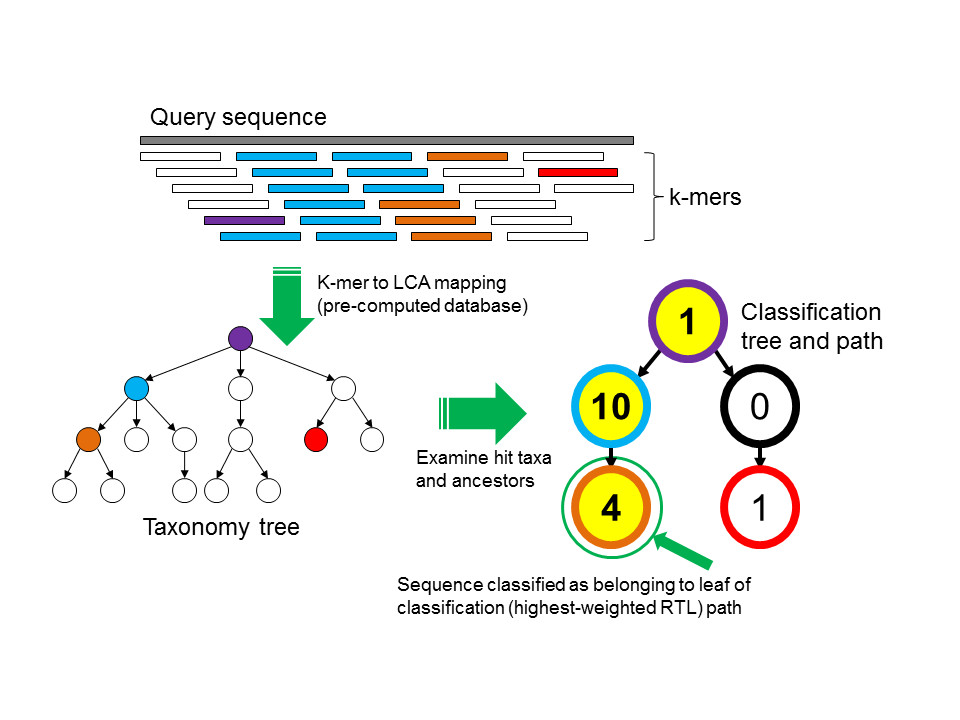
\includegraphics[width=\textwidth]{Work.jpg}
	\caption{Prikaza klasifikacije podataka}
	\label{Klasifikacija}
\end{figure}

Iz slike 3.2 se može vidjeti način rada algoritma. Nakon izračuna svih  k-mera ulaznog podatka, ti isti se pokušavaju klasificirati i izgraditi taksonomsko stablo pomocu vrijednosti najmanjeg zajedničkog pretka (LCA). To se izvodi pomoću predefinirane baze podataka. Upravo opisani dio rada je prikazana na slici 3.2 na u gornjem dijelu slike. Nakon toga se računaju težine za svaki čvor u stablu. Težine prestavljaju broj k-mera koji se podudaraju sa tim istim čvorom. Težine su predstavljene na slici 3.2 u desnom kutu.Ako postoji više različitih puteva koji imaju iste težine, tada se za iste ponovno računa najmanji zajednički predak te se pokušava dokučiti koji je pravi put, tj. koji od čvorova je pravi predak između listova koje smo tražili. Nadalje ako postoji više puteva ali oni nisu istih težina, tada se put do zajedničkog pretka uzima onaj put koji ima najveću težinu, tj. kojem odgovara najviše k-mera. To je prikazano na slici 3.2 u desnom kutu, gdje možemo vidjeti da se od dva različita puta bira onaj lijevi upravo zbog toga jer je njegov zbroj težina veći od desnog. S time se zaključuje da su težine proporcijonalne vjerojatnosti točnosti zadanog puta. 


\subsection{LCA(\textit{Lower Common Ancestor})}
LCA(\textit{Lower common ancestor}) je jedan od osnovnih algoritamskih problema u strukturama stabala.A označava pronalazak čvora u stablu koji je najudaljeniji od korijena stabla, te je zajednički čvorovima \textit{u} i \textit{v}. Prvu ideju i definiciju LCA dali su Alfred Aho, John Hopcroft i Jeffrey Ullman 1973. godine u svom radu \textit{On finding lowest common ancestors in trees}. Zbog svoje složenosti te raznolike primjenjivosti ovaj problem je još uvijek aktualan, te se i danas objavljuje mnogo članaka i radova na tu temu. U uvodu svog rada autori navode glavni problem koji LCA pokušava riješiti. Problem se navodi kao primanje informacija o novim osobama u određenim vremenskim intervali, te je pomoći zadanog algoritma potrebno točno odrediti sve veze između svakog novog čvori koji predstavlja danu informaciju,
\begin{figure}[!htbp]
	\centering
	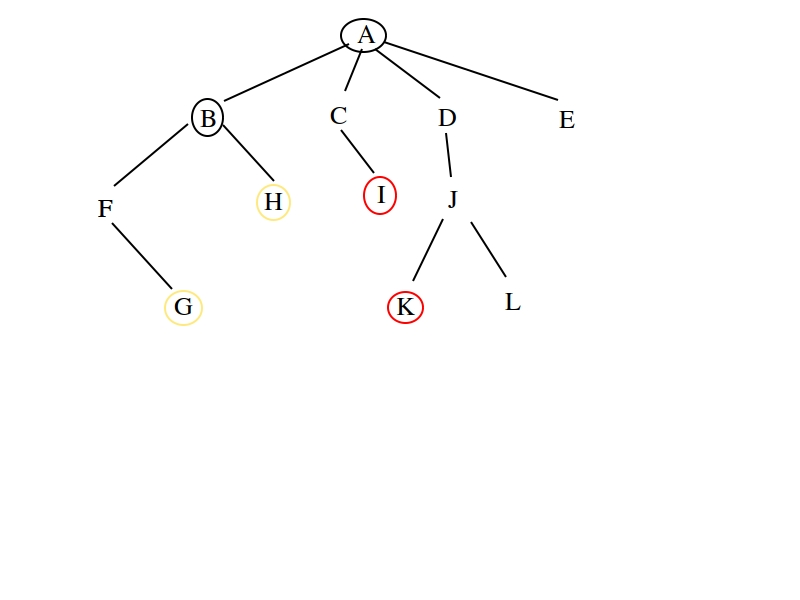
\includegraphics[width=\textwidth]{lca.jpg}
	\caption{Prikaz stabla i LCA vrijednosti}
	\label{LCA}
\end{figure}

Na slici 3.3 se nalazi prikaz strukture stabla te su bojama označeni listovi za koje želimo naći najmanjeg zajedničkog pretka (LCA). Crno obojani čvorovi su čvorovi koji su LCA tim dvama listovima. Tako je za listove H i G najmanji zajednički predak čvor B, dok je za listove I i K najmanji zajednički predak A. U radu \textit{On finding lowest common ancestors in trees} 1973. godine je predstavljen sljedeći pseudokod za određivanje najmanjeg zajedničkog pretka.
\newline
\newline
\begin{algorithm}[H]
	
	\SetAlgorithmName{Algoritam}{algoritam}{List of algoritam}
	
	procedure getancestor(u,i)\footnote[1]{A.V.Aho, J.E.Hopcroft, J.D.Ullman, \textbf{On finding lowest common ancestor in trees} \textit{ACM New York, NY, USA ©1973}}:\\

	
		\If{ancestor(u,i-1) = undefined then;}{
			ancestor(u,i) <- getancestor(getancestor(u,i-1),i-1)\;
		}
		resultis ancestor(u,i)\;
	\caption{Dohvaćanje pretka}
	\label{LCA algoritam 1}
\end{algorithm}

Algoritam 2 predstavlja metodu getancestor(u,i), koja prima čvor \textit{u} te dubinu \textit{i}. Funkcija dohvaća 2\^ i-tog pretka te ga stavlja u niz. \textit{Getancestor} se poziva tijekom traženja najmanjeg zajedničkog pretka. Ova metoda predstavlja očuvanje svih informacija o precima za jedan čvor. 
\newline
\begin{algorithm}[H]

	\SetAlgorithmName{Algoritam}{algoritam}{List of algoritam}
		procedure find(u,v,i,d)\footnote[2]{A.V.Aho, J.E.Hopcroft, J.D.Ullman, \textbf{On finding lowest common ancestor in trees} \textit{ACM New York, NY, USA ©1973}}:\\
		\eIf{i = 0}{
			resultis ancestor(u,0)\;
		}{
			\eIf{getancestor(u,i-1)=getancestor(v,i-1)}{
				resultis find(u,v,i-1,d)\;
			}{
				resultis find(getancestor(u,i-1),getancestor(v,i-1),min(i-1,|\_log(d-2\^(i-1))\_|),d-2\^(i-1))\;
			}
		}
	\caption{Pronalazak LCA}
	\label{LCA algorithm 2}
	
\end{algorithm}

Algoritam 3 predstavlja metodu koja pronalazi najmanjeg zajedničkog pretka za ulazne podatke \textit{u} i \textit{v} koji su na dubini \textit{d}. Početne pretpostavke su da je \textit{d} > 2 \^(i-1) te su im 2\^i-ti preci jednaki ili ne postoje. Zadana metoda radi na način da u svakom novom koraku smanjuje radni prostor koji pretražuje , tako da je put do najmanjeg zajedničkog pretka uvijek u zadanom prostoru. Gore navedene dvije metode omogućuju stvaranje metode koja osigurava pronalazak najmanjeg zajedničkog pretka uz pravilno biranje početnih uvjeta. Budući da se zadnji uvijek računa logaritamskom funkcijom, algoritam je optimiziran tako da se podaci predstavljaju kao binarne znamenke, te se u svakom koraku petlje pomiče za jedan bit dok ne dođe ko kraja.
\chapter{Algoritmi indeksiranja i pretrage}
\subsection{Minimizer - algoritam za reduciranje podataka}
Usporedba podataka je osnova moderne bioinformatike. Ona se danas temelji na metodi \textit{seed-and-extend}. Za svaki ulazni podatak se uzima samo jedan uzorak, te se on uspoređuje u bazi podataka. Ako se nađe poklapanje tada se taj uzorak proširuje na cijeli podatak te se ponovno uspoređuje. Da bi sve to funkcioniralo potrebno je uzeti uzorak za svaki podskup u jednom genomu, što , za kompleksnije genome, zauzima jako puno memorije.Na ideju rješenja su došli Michael Roberts, Wayne Hayes, Brian R. Hunt, Stephen M. Mount i James A. York u svom radu \textit{Reducing storage requirements for biological sequence comparison}. Koristi se isti način rada, tj.\textit{seed-and-extend}, uz razliku da se ne uzimaju svi uzorci, nego samo mali podskup jedinstvenih, nazvanih "minimizer-i".
\\ Navedeni algoritam sažimanja se koristi i u Kraken bazi podataka, te ju uvelike smanjuje i pospješuje brzinu izvođenja. Prilikom kreiranja MiniKraken baze podataka se koristi isti način rada, uz razliku da se odbacuje samo određeni postotak prvih i zadnjih vrijednosti. Da bi kontejneri u kojima su sadržani podaci s istim minimizer vrijednostima zadržao svojstvo kolekcije, potrebno je da su ti isti podaci normalno distribuirani, što se postiže brisanjem pola bitova prilikom ispitivanja jednakosti. S ciljem pospješenja brzine izvođenja, jer svako računanje minimizer vrijednosti je relativno skupo, prilikom klasifikacije podatka koristi se onaj kontejner koji je korišten prije, te ako k-meri nisu nađeni u njemu, računa se minimizer vrijednost. Ako je minimizer vrijednost jednaka kao u kontjerneru zaključuje se da se podatak ne može klasificirati, inače se pozicionira u dani kontejner te se ponovno vrši pretraga.

Postije dvije vrste minimizer-vrijednosti: unutarnje i vanjske. Svakoj od njih je srž računanja isti, tj. za ulazni niz se računaju svi njegovi k-meri za zadani k, te se iz njih tada bira onaj k-mer koji je leksikografski najmanji. 

\begin{figure}[htbp]
	\centering
	
	\begin{tabular}{l|l|llllllll|}
		\multicolumn{2}{l|}{Pozicija:}                                                                                       &  & 1 & 2 & 3 & 4          & 5          & 6          & 7 \\ \hline
		\multicolumn{2}{l|}{Ulazni niz:}                                                                                     &  & 2 & 3 & 1 & 0          & 3          & 4          & 3 \\ \hline
		\multicolumn{2}{l|}{\multirow{5}{*}{\begin{tabular}[c]{@{}l@{}}k-meri\\ s\\ podebljanim\\ minimizerom\end{tabular}}} &  & 2 & 3 & 1 &            &            &            &   \\
		\multicolumn{2}{l|}{}                                                                                                &  &   & 3 & 1 & 0          &            &            &   \\
		\multicolumn{2}{l|}{}                                                                                                &  &   &   & 1 & 0          & 3          &            &   \\
		\multicolumn{2}{l|}{}                                                                                                &  &   &   &   & \textbf{0} & \textbf{3} & \textbf{4} &   \\
		\multicolumn{2}{l|}{}                                                                                                &  &   &   &   &            & 3          & 4          & 3 \\ \hline
	\end{tabular}
	\caption{K-meri ulaznog niza s minimizer-om}
	\label{Minimizer}
\end{figure}

Slika 4.1 prikazuje način odabira minimizera za ulazni niz. Ulazni niz je podjeljen na 3-mere , a za računanje minimizer-a se koristi prozor od 5 k-mera. Korištenje prozora znači da se samo u 5 k-mera odjednom traži minimizer vrijednost. Budući da je \textit{034} leksikografksi najmanji podniz on se uzima kao zadani minimizer. Algoritam minimizer nam garantira da će dva niza koja su ista sadržavati barem jednu istu minimizer vrijednost.
\subsection{Binarno pretraživanje}
Za pretraživanje svakog kontejnera se koristi binarno pretraživanje. Binarno pretraživanje je jedan od osnovnih algoritama u računalnoj znanosti. Glavni zadatak algoritma je pronalazak vrijednosti u sortiranom nizu. Osnovna i glavna pretpostavka jest da je niz sortiran, u suprotnom sam algoritam nema smisla.
\newline
\newline
\begin{algorithm}[H]
	\SetAlgorithmName{Algoritam}{algoritam}{List of algoritam}
	binarno\_pretraživanje(niz,cilj):\\
	lo = 1, hi = size(niz)\;
	\While{lo <= hi}{
		mid = lo + (hi - lo) / 2\;
		\eIf{niz[mid] == cilj}{
			return mid\;
		}{
			\eIf{niz[mid] < cilj}{
				lo = mid + 1\;	
			}{
				hi = mid + 1\;
			}
		}
	}
	\caption{Binarno pretraživanje}
	\label{BinarnoP}
\end{algorithm}

Inicijalno je radni prostor binarnog pretraživanja cijeli ulazni niz. Tada se pozicionira na sredinu tog niza, te se ispituje je li vrijednost na sredini jednaka onoj koju mi tražimo. Ako je rezultat potvrdan izlazimo iz petlje te vraćamo poziciju te vrijednosti. U protivnom se ispituje odnos tražene vrijednosti i one koja je na sredini. Ako je vrijednost na sredini manja od tražene radni prostor postavljamo na onu polovicu koja se nalazi desno od indeksa, tj. prelazimo u  polovicu koja sadrži veće vrijednosti, u suprotnom se pozicioniramo na manju polovicu. Složenost binarnog pretraživanja je O(logN). Logaritam je sporo rastuća funkcija, stoga je binarno pretraživanje jako efikasan algoritam. Kao primjer za pretragu imenika od milion imena, pomoću binarnog pretraživanja bismo pronašli traženu vrijednost u najviše 21 korak.


\chapter{Pseudokod i razrada algoritma}
Riješenja navedenog problema o korištenju baze podataka na ograničenim resursima se sastoji iz nekoliko dijelova. Za početak je potrebno podjeliti bazu podataka na manje cjeline, zatim je potrebno ostvariti straničenje na tim cjelinama.
\subsubsection{Problemi kod korištenja Kraken baze podataka}

Iako je prvotna ideja bila koristiti Kraken bazu podataka, te je algoritam i osmišljen upravo za nju, zbog tehničkih problema se moralo odustati od te ideje. Sama baza podataka je u nepodržanom formatu za bilo koji preglednik baze podataka koji sam uspio naći, a proučavanjem izvornog koda Kraken alata se nije moglo puno zaključiti. Kod je slabo zakomentiran te je veliki problem snaći se u takvom okruženju. Stoga se za daljnji rad koristi jednostavna baza podataka od par stotina kilobayta.

\subsubsection{Podjela baze podataka}
Iz gore navedenih razloga odlučeno je prezentirati rad algoritma, te samu raspodjelu baze podataka na uzorku baze podataka\footnote{http://www.sqlitetutorial.net/sqlite-sample-database/}.
\begin{figure}[!htbp]
	\centering
	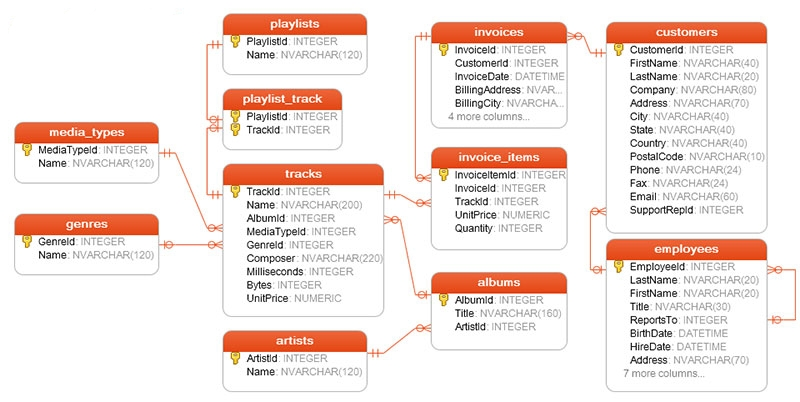
\includegraphics[width=\textwidth]{sqlite-sample-database-color.jpg}
	\caption{Prikaz korištene baze podataka}
	\label{Db}
\end{figure}
Baza podataka je sqlite3 tipa, te se u izvornom kodu programa koristi paket sqlite3.\\
Podjela baze podataka na cjeline je ostvarena bash skriptom, koja na pomoću sqlite3 naredbi iz zadane baze podataka kreira datoteku koja sadrži sql upite koji stvaraju kostur baze podataka, tj. stvara zadani broj identičnih baza podataka kao originalna ali bez ijednog podatka u sebi.\\ Budući da je već gotovu bazu podataka gotovo nemoguće podijeliti na funkcionalne baze, morao se je koristiti pristup gdje se ista pretvara u niz sql upita.

\begin{algorithm}[H]
	\SetAlgorithmName{Algoritam}{algoritam}{List of algoritam}
		\If{postoji schema.sql}{izbriši schema.sql\;}
		\If{postoji dump.sql}{izbriši dump.sql\;}
		sqlite3 imebaze .schenm -> schema.sql\;
		sqlite3 imebaze .dump -> dump.sql\;
	\caption{Podjela baze podataka}
	\label{PodjelaBp}
\end{algorithm}

Gore navedenim dijelom koda se stvaraju datoteke schema.sql i dump.sql. Schema.sql sadrži SQL upite koji stvaraju strukturu originalne baze podataka, a dump.sql se sastoji od SQL upita koji pune bazu podataka podacima iz originalne baze podataka.
\\Budući da želimo bazu podataka podjeliti na cjeline potrebno je file dump.sql podjeliti na onoliko fileova koliko želimo da imamo baza podataka. U svrhe demonstracije rješenja dump.sql je podjeljen u 5 cjelina koje su slijedno razdvojene, tj. ne prate nikakvu logiku koja bi možda pospješila pretragu, ili čak imala nekog smisla. \\Za Kraken bazu podataka se može koristiti datoteka koja sadrži indekse svakog kontejnera , te možemo dobiti baze podataka koje sadrže samo one podatke čiji k-meri imaju jednake minimizer vrijednosti. Iza tog problema se krije ne jako zahtjevna logika koju relativno lako možemo realizirati u bash skripti.
\\Time ne završava cijepanje baze podataka na manje dijelove, naime potrebno je kreirati svaku bazu podataka te unijeti podatke u svaku zasebno. Iz dump.sql datoteke je dobiveno 6 dump.split.000x.sql datoteka , koje će svaka za sebe graditi bazu podataka. Kako smo datoteku podjelili pomoću jednostavne \textit{split} naredbe u bash-u dobivene datoteke nisu pravilno konfigurirane za kreiranje. Stoga je potrebno , ako ne postoji, na početku svake datoteke upisati SQL naredbu  \textit{BEGIN TRANSACTION}, te na kraju iste , opet ako ne postoji, upisati naredbu \textit{COMMIT}. To je izvedeno sljedećim dijelom bash skripte.

\begin{algorithm}[H]
	\SetAlgorithmName{Algoritam}{algoritam}{List of algoritam}
	\For{svaku datoteku u direktoriju}{
		\If{"BEGIN TRANSACTION" se ne nalazi na početku datoteke}{
			dodaj\_BEGIN\_TRANSACTION\_na\_početak\;
		}
		\If{"COMMIT" se ne nalazi na kraju datoteke}{
			dodaj\_COMMIT\_na\_kraj\;
		}
	}
	\caption{Osposobljavanje dump datoteka}
	\label{DumpBp}
\end{algorithm}

Naposlijetku je potrebno kreirati bazu podataka. To se radi na način da se za svaku dump.split.000x.sql datoteku kreira baza podataka koja sadrži samo kostur originalne baze, te se u nju tada pomoću navedene datoteke ubacuju podaci. Na kraju izvedbe zadanog programa smo dobili 6 baza podataka koje zajedno imaju sve podatke koje je zadržavala originalna baza podataka.

\subsubsection{Straničenje}
Kako,zbog tehničkih poteškoća, nismo radili sa Kraken ili MiniKraken bazom podataka za prezentaciju algoritma straničenja koristit će se jednostavni SQL upit koji želi dohvatiti sve podatke za neku tablicu. Algoritam straničenja je prvotno bio osmišljen u verziji koja bi bila dosta brža, ali za ovaj rad je obrađeno samo standardno straničenje.

	\begin{algorithm}[H]
		\SetAlgorithmName{Algoritam}{algoritam}{List of algoritam}
		\For{ima podataka u listi}{
			\For{i < broj\_baza\_podataka}{
				otvori bazu podataka()\;
				pozovi SQL upit nad bazom podataka()\;
				zatvori bazu podataka()\;	
			}
		}
		\caption{Algoritam straničenja}
		\label{Stranicenje}
	\end{algorithm}

Gore navedeni pseudokod predstavlja algoritam koji je implementiran za potrebe ovoga rada. Poboljšana verzija bi se sastojala od toga da se za ulazni podataka izračuna indeks te se otvori i pretrači samo baza podataka koja može sadržavati zadani indeks. Taj algoritam je predstavljen sljedećim pseudokodom.
\newline
	\begin{algorithm}[H]
		\SetAlgorithmName{Algoritam}{algoritam}{List of algoritam}
		\For{ima podataka u listi}{
			izračunaj indeks za ulazni podatak();
			\eIf{otvorena baza je istog indeksa ko podatak}{
				pozovi SQL upit nad bazom podataka()\;
			}{
				
				zatvori bazu podataka()\;
				pozovi SQL upit nad bazom podataka()\;
				otvori bazu podataka()\;
			}
		}
		\caption{Poboljšani algoritam straničenja}
		\label{Stranicenje2}
	\end{algorithm}

Testiranje za zadanu bazu podataka daje obećavajuće rezultate. Svi podaci su ostali sačuvani, te je za tablicu imena \textit{albums}, SQL upitom SELECT * FROM albums rezultat prikazao sve podatke koji se nalaze u originalnoj bazi.
\chapter{Analiza učinkovitosti rješenja}
Zbog nemogućnosti korištenja Kraken i MiniKraken baze podataka testovi koje je moguće provesti za zadani algoritam su ograničeni. Prvi provedeni test je izveden naredbom SELECT * FROM playlists te je utvrđeno da si svi podaci ostali sačuvani, te da callback metoda ,koja je zaslužena za ispisivanje svih dobivenih podataka, nema nikakvih problema s njihovom interpretancijom. 
\newline
\begin{figure}[hbp]
	\begin{lstlisting}
static int callback(void *data, int argc, char **argv,char **azColName){
	int i;
	fprintf(stderr, "%s:", (const char*)data);
	for(i=0; i<argc; i++){
		printf("%s=%s\n", azColName[i],argv[i] ? argv[i] : "NULL");
	}
	printf("\n");
	return 0;
}
	\end{lstlisting}
\end{figure}

S obzirom na vrijeme izvođenja u samom početku se moglo zaključiti da će program raditi sporije, pogotovo na većim bazama koje će se morati učitati u RAM. Međutim cilj ovog rješenja je osposobljavanje na rad, ali i spremnost na nešto sporiji rad. Naravno sve se još da optimizirati raznim algoritmima pretrage te korištenjem indeksa za interpretaciju i dohvaćanje raznih baza podataka. Jedan od glavnih problema ovog pristupa je bio kako uspješno već gotovu bazu podataka raspodjeliti u manje a da podaci ostanu kontinuirani i indeksi na u svim tablicama ostanu očuvani, što je uspješno odrađeno. Iako neobičan, pristup problemu tako da se cijela baza podataka pretvori u niz SQL upita se pokazao kao jako dobar, te će se zasigurno koristiti u mom daljnjem istraživanju i pokušavanju rješenja navedenog problema. Budući da je baza podataka jako mala nije se mogao provesti smislen test postrošnje vremena koji će potkrijepiti gore navedenu teoriju.
\subsection{Za budućnost}
U budućem radu ću se više osloniti na implementaciju rješenja konkretno na Kraken bazu podataka, koja je do sada predstavljala veliki problem. Pokušat kontaktirati autore samog alata se u dogovoru s njim raditi na rješavanju, po mom mišljenju, jednog jako zanimljivog problema koji može poboljšati Kraken do krajnjih granica. Budući rad podrazumjeva dolaženje do podataka koji se nalaze u Kraken bazi podataka, te podjela iste baze na manje cjeline. Razlika od dosadašnjeg rada je da se baza podataka neće dijeliti na bilo koje cjeline, nego će jednu novu bazu podataka činiti jedan kontejner jedinstvenog minimizera. Tada u implementaciju nastupa implementiranje straničenja podataka, poboljšanje samog straničenja korištenjem liste indeksa.
\chapter{Zaključak}
Bioinformatika kao interdisciplinarna znanost koja spaja više prirodno-matematičkih znanosti otvara vrata za ozbiljnu suradnju znanstvenika s tih područja. Kroz veliki razvitak u zadnjim desetljećima bioinformatika se razvila u znanost koja uspjeva napraviti mnogo toga. U zadnjem desetljeću se uspješno mapirao cijeli genom čovjeka. Upravo zbog svog razvitka jako brzo su se počeli pojavlivati programi koji su mnogo doprinjeli cijeloj toj priči. Jedan od tih je i Kraken. Svojom izrazitom preciznošću se primiče svojevrsnom vrhuncu u točnosti klasifikacije genoma, te svojom brzinom izvođenja se odmiče od većine drugih alata. Uspješno spaja nekoliko algoritama za indeksiranje, pretragu te klasifikaciju podataka pomoću stabla. Za klasificiranje podataka se koristi LCA algoritam, te za indeksiranje i pretragu baze podataka Minimizer algoritam. Upravo kod baze podataka nastupa problem kojim se bavi ovaj rad. Kako bazu od nekoliko desatak GB ubaciti u RAM koji je samo nekoliko GB. Idejom raspodjele baze podataka te stranišenjem tih baza se pokušalo približiti rješenju, te se ovim radom to i uspjelo. Rana testiranja, koja naposlijetku , zbog tehničkih problema, se niju uspjela odviti na Kraken bazi podataka, su pokaza jednu od najbitnijih značajki koja se morala zadržati, a to je kontinuiranost podataka te indeksa istih. U daljnjem radu na ovom problemu pokušat će se sve to implementirati na prvotno namjenjenu bazu podataka, te ispitati ponašanje istog.

\bibliography{literatura}
\bibliographystyle{fer}
\nocite{Kraken}
\nocite{Bigdatabases}
\nocite{minim}
\nocite{jellyfish}
\nocite{lca1}
\nocite{lca3}
\nocite{lca2}


\begin{sazetak}
Straničenje velike baze podataka se odvija u dva koraka. Prvi je raspodjeljivanje baze na manje cjeline(baze podataka manjeg memorijskog kapaciteta). On je ostvaren pomoću bash skripte koja uz sqlite3 naredbe uspjeva napraviti kostur originalne baze te SQL upite za punjenje baze podacima.\\
Drugi  korak je samo straničenje koje se odvija jednostavnom for petljom koja iterira po svim bazama te traži podatak koji želimo obraditi. Za nastavak i poboljšanje straničenja se može uvesti lista indeksa baza podataka te se jednostavnim pretraživanjem liste može utvrditi samo jedna baza podataka koju trebamo učitati.

\kljucnerijeci{straničenje, baza podataka, SQL upit, Kraken, metagenom, k-mer, LCA, minimizer}
\end{sazetak}

% TODO: Navedite naslov na engleskom jeziku.
\engtitle{Algorithm for Paging Large-Scale Genome Database}
\begin{abstract}
Paging of large-scale database contains two steps. First one is splitting database into smaller units(databases that contains less memory). It is done by bash script that using sqlite3 commands manages to create skeleton of original database, and creates SQL commands for filling database with data.
\\Second step is paging itself that is happening by simple for loop which iterates over all databases and searches data that we want to process. For continuation and improvement of paging one can use index list and by simple search of that list can determine only one database that one needs to load.

\keywords{paging, database, SQL command, Kraken, metagenom, k-mer, LCA, minimizer}
\end{abstract}

\begin{appendices}
	\chapter{Upute za korištenje programske potpore}
	Upute za korištenje programske potpore:
	\\Za koristiti programsku podršku potrebno je raditi na nekoj od Linux distribucija, te ista mora sadržavati instalirane sqlite3 i sqlite3-devel pakete
	\\Za rad sa izvršnim programo preuzeti direktorij koji sadrži sve zadane komponente
	\\Pozicionirati se u direktorij Database
	\\Pokrenuti skriptu splitScript.sh sa argumentima imena baze podataka te brojem baza koje želimo napraviti
	\\Dump.sql i schema.sql će biti spremljeni u trenutni direktorij
	\\Baze podataka će biti spremljene u direktorij Databases dok će raspodjeljena dump datoteka biti u Splitted direktoriju
	\\Pokrenuti Makefile
	\\Pokrenuti izvršni program sa argumentom broja baza koje želimo koristiti
\end{appendices}

\end{document}
